\documentclass[notheorems,mathserif,table,compress]{beamer}  %dvipdfm选项是关键,否则编译统统通不过
%%------------------------常用宏包------------------------
%%注意, beamer 会默认使用下列宏包: amsthm, graphicx, hyperref, color, xcolor, 等等
\usepackage{fontspec,xunicode,xltxtra}  % for XeTeX
\usepackage{comment}
\usepackage{fancybox}
\usepackage{indentfirst}%%段前空格
\usepackage{subfigure}  %%图形或表格并排排列
%%------------------------ThemeColorFont------------------------
%% Presentation Themes
% \usetheme[<options>]{<name list>}
\usetheme{Madrid}
%% Inner Themes
% \useinnertheme[<options>]{<name>}
%% Outer Themes
% \useoutertheme[<options>]{<name>}
\useoutertheme{miniframes} 
%% Color Themes 
% \usecolortheme[<options>]{<name list>}
%% Font Themes
% \usefonttheme[<options>]{<name>}
\setbeamertemplate{background canvas}[vertical shading][bottom=white,top=structure.fg!7] %%背景色, 上25%的蓝, 过渡到下白.
\setbeamertemplate{theorems}[numbered]
\setbeamertemplate{navigation symbols}{}   %% 去掉页面下方默认的导航条.
\usepackage{zhfontcfg}
%\setsansfont[Mapping=tex-text]{文泉驿正黑}  %% 需要fontspec宏包
     %如果装了Adobe Acrobat,可在font.conf中配置Adobe字体的路径以使用其中文字体
     %也可直接使用系统中的中文字体如SimSun,SimHei,微软雅黑 等
     %原来beamer用的字体是sans family;注意Mapping的大小写,不能写错
     %设置字体时也可以直接用字体名,以下三种方式等同:
     %\setromanfont[BoldFont={黑体}]{宋体}
     %\setromanfont[BoldFont={SimHei}]{SimSun}
     %\setromanfont[BoldFont={"[simhei.ttf]"}]{"[simsun.ttc]"}
%%------------------------MISC------------------------
\graphicspath{{figures/}}         %% 图片路径. 本文的图片都放在这个文件夹里了.
%%------------------------正文------------------------
\begin{document}
\XeTeXlinebreaklocale "zh"         % 表示用中文的断行
\XeTeXlinebreakskip = 0pt plus 1pt % 多一点调整的空间
%%----------------------------------------------------------
%% This is only inserted into the PDF information catalog. Can be left
%% out.
%%%
%% Delete this, if you do not want the table of contents to pop up at
%% the beginning of each subsection:
\begin{comment}
\AtBeginSection[]{                              % 在每个Section前都会加入的Frame
  \frame<handout:0>{
    \frametitle{插入一张图片}\small
    \tableofcontents[current,currentsubsection]
  }
}
\AtBeginSubsection[]                            % 在每个子段落之前
{
  \frame<handout:0>                             % handout:0 表示只在手稿中出现
  {
    \frametitle{下一节内容}\small
    \tableofcontents[current,currentsubsection] % 显示在目录中加亮的当前章节
  }
}
\end{comment}
%%----------------------------------------------------------
\title[小练习]{\LaTeX 小练习}
\author[常琳]{常琳}
  %\hspace{2.28em}导师~~\textcolor{olive}{姬光荣}~教授}
%\institute[中国海洋大学]{\small\textcolor{violet}{中国海洋大学~~信息科学与工程学院}}
\date{\today}
%\titlegraphic{\vspace{-6em}\includegraphics[height=7cm]{ouc}\vspace{-6em}}
\frame{ \titlepage }
%%----------------------------------------------------------
%\section*{目录}
\frame{\frametitle{目录}\tableofcontents}
%%----------------------------------------------------------
\section{插入一张图片}
\begin{frame}
  \frametitle{插入一张图片}
  \begin{figure}[!ht]
  \centering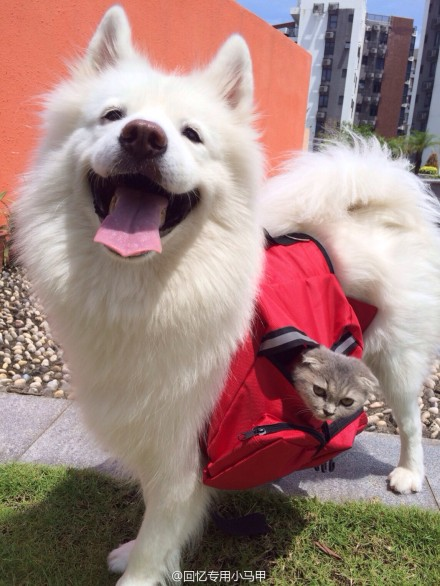
\includegraphics[width=1.5in]{dog.jpg}
  \caption{一只狗}
  \end{figure}
\end{frame}
%-----------------------------------------------------------------------
\section{三种形式的使用}
\begin{frame}
  \frametitle{三种形式的使用}
  \subsection{itemize}
本周学习内容:
\begin{itemize}
\item \LaTeX 的应用。
\item 学习的方法,终端的一些快捷操作方法。
\item 学习GitHub的使用,包括更新本地仓库,上传文件到GitHub上。
\end{itemize}
 \subsection{description}
\begin{description}
\item[首先] 明白一些基本概念,如文件跟踪、文件的三种状态等。
\item[然后] 首次克隆文件到本地仓库或者上传文件到一个新的仓库。
\item[最后] 如何更新仓库,如何添加描述。
\end{description}
\subsection{enumerate}
本周学习成果与问题:
\begin{enumerate}
\item GitHub的基本操作已经掌握。
\item \LaTeX 的排版还是无法独立完成,排版不够美观。
\end{enumerate}
\end{frame}
%----------------------------------------------------------------------
\section{三个段落排版}
\begin{frame}
\frametitle{三个段落排版}
  \hspace{0.3in}beamer类型下的段落排版不同于article,在这种类型下不适合出现大段大段的文字。


  \hspace{0.3in}速度速度没地方是你就不懂覅速度速度没地方是你就不懂覅速度速度没地方是你就不懂覅速度速度没地方是你就不懂覅速度速度没地方是你就不懂覅速度速度没地方是你就不。


  \hspace{0.25in} 速度速度没地方是你就不懂覅速度速度没地方是你就不懂覅速度速度没地方是你就不懂覅速度速度没地方是你就不懂覅速度速度没地方是你就不懂覅速度速度没地方是你就不懂覅速度速度没地方。
\end{frame}
%------------------------------------------------------------------------
\section{插入两张并列的图片}
\begin{frame}
  \frametitle{插入两张并列的图片}
如何快速调整两张图片的大小与位置,使排版合理。
\begin{figure}[!ht]
  \begin{minipage}[t]{0.5\textwidth}	
  \centering
  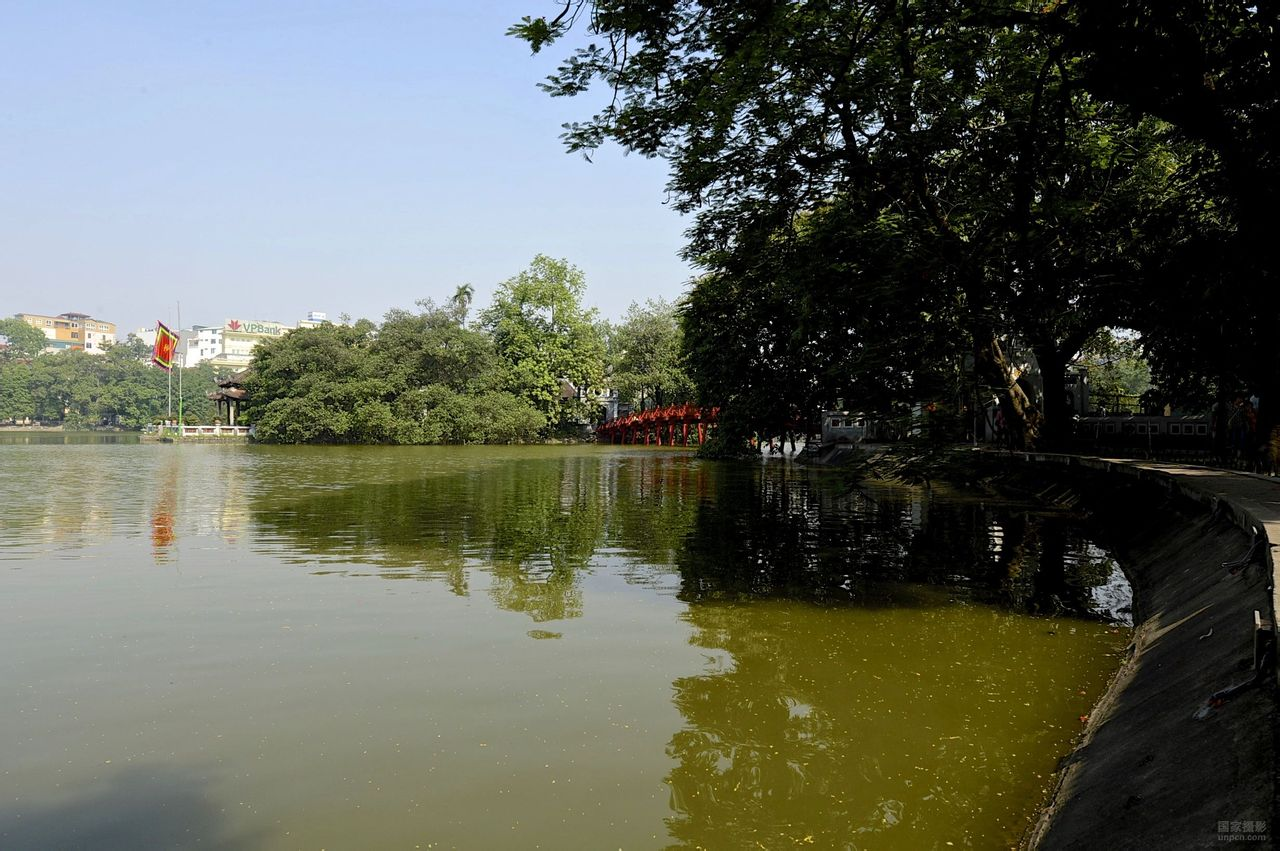
\includegraphics[width=2.2in]{view.jpg}
  \caption{河内风景}
  \end{minipage}
  \begin{minipage}[t]{0.4\textwidth}
  \centering
  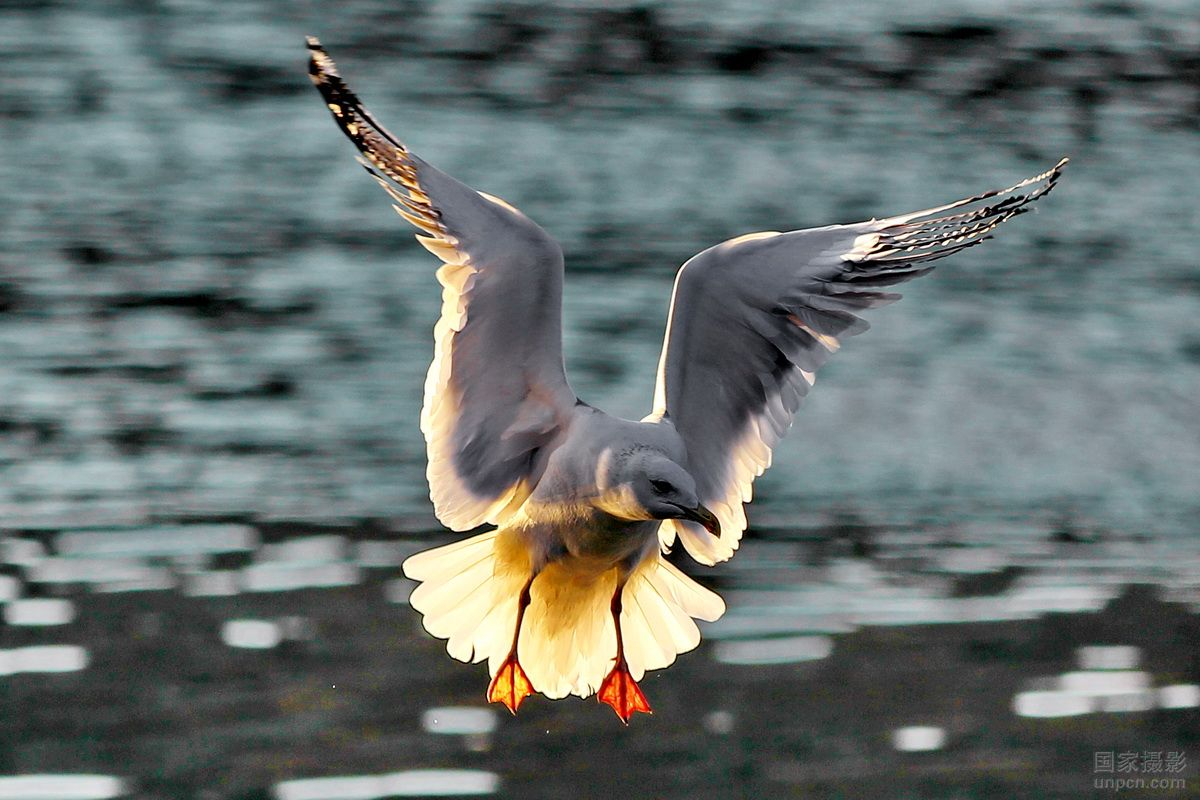
\includegraphics[width=2.2in]{bird.jpg}%如何快速调整两张图像大小与位置?
  \caption{觅食}
  \end{minipage}
  \end{figure} 

\end{frame}
%----------------------------------------------------------------------
\section{插入公式}
\begin{frame}
  \frametitle{插入公式}
 $$y=\sum_{i=0}^{n}\frac{x^2+a^2}{b^2}$$

 $$\lim_{n \to \infty}
\sum_{k=0}^n \frac{1}{k^2}
= \frac{\pi^2}{6}$$
\end{frame}
\end{document}
